\documentclass[twoside]{book}

% Packages required by doxygen
\usepackage{fixltx2e}
\usepackage{calc}
\usepackage{doxygen}
\usepackage[export]{adjustbox} % also loads graphicx
\usepackage{graphicx}
\usepackage[utf8]{inputenc}
\usepackage{makeidx}
\usepackage{multicol}
\usepackage{multirow}
\PassOptionsToPackage{warn}{textcomp}
\usepackage{textcomp}
\usepackage[nointegrals]{wasysym}
\usepackage[table]{xcolor}

% Font selection
\usepackage[T1]{fontenc}
\usepackage[scaled=.90]{helvet}
\usepackage{courier}
\usepackage{amssymb}
\usepackage{sectsty}
\renewcommand{\familydefault}{\sfdefault}
\allsectionsfont{%
  \fontseries{bc}\selectfont%
  \color{darkgray}%
}
\renewcommand{\DoxyLabelFont}{%
  \fontseries{bc}\selectfont%
  \color{darkgray}%
}
\newcommand{\+}{\discretionary{\mbox{\scriptsize$\hookleftarrow$}}{}{}}

% Page & text layout
\usepackage{geometry}
\geometry{%
  a4paper,%
  top=2.5cm,%
  bottom=2.5cm,%
  left=2.5cm,%
  right=2.5cm%
}
\tolerance=750
\hfuzz=15pt
\hbadness=750
\setlength{\emergencystretch}{15pt}
\setlength{\parindent}{0cm}
\setlength{\parskip}{3ex plus 2ex minus 2ex}
\makeatletter
\renewcommand{\paragraph}{%
  \@startsection{paragraph}{4}{0ex}{-1.0ex}{1.0ex}{%
    \normalfont\normalsize\bfseries\SS@parafont%
  }%
}
\renewcommand{\subparagraph}{%
  \@startsection{subparagraph}{5}{0ex}{-1.0ex}{1.0ex}{%
    \normalfont\normalsize\bfseries\SS@subparafont%
  }%
}
\makeatother

% Headers & footers
\usepackage{fancyhdr}
\pagestyle{fancyplain}
\fancyhead[LE]{\fancyplain{}{\bfseries\thepage}}
\fancyhead[CE]{\fancyplain{}{}}
\fancyhead[RE]{\fancyplain{}{\bfseries\leftmark}}
\fancyhead[LO]{\fancyplain{}{\bfseries\rightmark}}
\fancyhead[CO]{\fancyplain{}{}}
\fancyhead[RO]{\fancyplain{}{\bfseries\thepage}}
\fancyfoot[LE]{\fancyplain{}{}}
\fancyfoot[CE]{\fancyplain{}{}}
\fancyfoot[RE]{\fancyplain{}{\bfseries\scriptsize Generated by Doxygen }}
\fancyfoot[LO]{\fancyplain{}{\bfseries\scriptsize Generated by Doxygen }}
\fancyfoot[CO]{\fancyplain{}{}}
\fancyfoot[RO]{\fancyplain{}{}}
\renewcommand{\footrulewidth}{0.4pt}
\renewcommand{\chaptermark}[1]{%
  \markboth{#1}{}%
}
\renewcommand{\sectionmark}[1]{%
  \markright{\thesection\ #1}%
}

% Indices & bibliography
\usepackage{natbib}
\usepackage[titles]{tocloft}
\setcounter{tocdepth}{3}
\setcounter{secnumdepth}{5}
\makeindex

% Hyperlinks (required, but should be loaded last)
\usepackage{ifpdf}
\ifpdf
  \usepackage[pdftex,pagebackref=true]{hyperref}
\else
  \usepackage[ps2pdf,pagebackref=true]{hyperref}
\fi
\hypersetup{%
  colorlinks=true,%
  linkcolor=blue,%
  citecolor=blue,%
  unicode%
}

% Custom commands
\newcommand{\clearemptydoublepage}{%
  \newpage{\pagestyle{empty}\cleardoublepage}%
}

\usepackage{caption}
\captionsetup{labelsep=space,justification=centering,font={bf},singlelinecheck=off,skip=4pt,position=top}

%===== C O N T E N T S =====

\begin{document}

% Titlepage & ToC
\hypersetup{pageanchor=false,
             bookmarksnumbered=true,
             pdfencoding=unicode
            }
\pagenumbering{alph}
\begin{titlepage}
\vspace*{7cm}
\begin{center}%
{\Large Splendor \\[1ex]\large 1.\+1 }\\
\vspace*{1cm}
{\large Generated by Doxygen 1.8.14}\\
\end{center}
\end{titlepage}
\clearemptydoublepage
\pagenumbering{roman}
\tableofcontents
\clearemptydoublepage
\pagenumbering{arabic}
\hypersetup{pageanchor=true}

%--- Begin generated contents ---
\chapter{Namespace Index}
\section{Packages}
Here are the packages with brief descriptions (if available)\+:\begin{DoxyCompactList}
\item\contentsline{section}{\mbox{\hyperlink{namespace_splendor}{Splendor}} }{\pageref{namespace_splendor}}{}
\item\contentsline{section}{\mbox{\hyperlink{namespace_splendor_1_1_properties}{Splendor.\+Properties}} }{\pageref{namespace_splendor_1_1_properties}}{}
\end{DoxyCompactList}

\chapter{Hierarchical Index}
\section{Class Hierarchy}
This inheritance list is sorted roughly, but not completely, alphabetically\+:\begin{DoxyCompactList}
\item \contentsline{section}{Splendor.\+Card}{\pageref{class_splendor_1_1_card}}{}
\item \contentsline{section}{Splendor.\+Connection\+DB}{\pageref{class_splendor_1_1_connection_d_b}}{}
\item Form\begin{DoxyCompactList}
\item \contentsline{section}{Splendor.\+frm\+Splendor}{\pageref{class_splendor_1_1frm_splendor}}{}
\end{DoxyCompactList}
\item \contentsline{section}{Splendor.\+Player}{\pageref{class_splendor_1_1_player}}{}
\end{DoxyCompactList}

\chapter{Class Index}
\section{Class List}
Here are the classes, structs, unions and interfaces with brief descriptions\+:\begin{DoxyCompactList}
\item\contentsline{section}{\mbox{\hyperlink{class_splendor_1_1_card}{Splendor.\+Card}} \\*class \mbox{\hyperlink{class_splendor_1_1_card}{Card}} \+: attributes and methods to deal with a card }{\pageref{class_splendor_1_1_card}}{}
\item\contentsline{section}{\mbox{\hyperlink{class_splendor_1_1_connection_d_b}{Splendor.\+Connection\+DB}} \\*contains methods and attributes to connect and deal with the database }{\pageref{class_splendor_1_1_connection_d_b}}{}
\item\contentsline{section}{\mbox{\hyperlink{class_splendor_1_1frm_splendor}{Splendor.\+frm\+Splendor}} \\*manages the form that enables to play with the \mbox{\hyperlink{namespace_splendor}{Splendor}} }{\pageref{class_splendor_1_1frm_splendor}}{}
\item\contentsline{section}{\mbox{\hyperlink{class_splendor_1_1_player}{Splendor.\+Player}} \\*class \mbox{\hyperlink{class_splendor_1_1_player}{Player}} \+: attributes and methods to deal with a player }{\pageref{class_splendor_1_1_player}}{}
\end{DoxyCompactList}

\chapter{Namespace Documentation}
\hypertarget{namespace_splendor}{}\section{Splendor Namespace Reference}
\label{namespace_splendor}\index{Splendor@{Splendor}}
\subsection*{Classes}
\begin{DoxyCompactItemize}
\item 
class \mbox{\hyperlink{class_splendor_1_1_card}{Card}}
\begin{DoxyCompactList}\small\item\em class \mbox{\hyperlink{class_splendor_1_1_card}{Card}} \+: attributes and methods to deal with a card \end{DoxyCompactList}\item 
class \mbox{\hyperlink{class_splendor_1_1_connection_d_b}{Connection\+DB}}
\begin{DoxyCompactList}\small\item\em contains methods and attributes to connect and deal with the database \end{DoxyCompactList}\item 
class \mbox{\hyperlink{class_splendor_1_1frm_splendor}{frm\+Splendor}}
\begin{DoxyCompactList}\small\item\em manages the form that enables to play with the \mbox{\hyperlink{namespace_splendor}{Splendor}} \end{DoxyCompactList}\item 
class \mbox{\hyperlink{class_splendor_1_1_player}{Player}}
\begin{DoxyCompactList}\small\item\em class \mbox{\hyperlink{class_splendor_1_1_player}{Player}} \+: attributes and methods to deal with a player \end{DoxyCompactList}\item 
class {\bfseries Program}
\end{DoxyCompactItemize}
\subsection*{Enumerations}
\begin{DoxyCompactItemize}
\item 
\mbox{\Hypertarget{namespace_splendor_abc955fe800ad5f701f777df0a2a29dc2}\label{namespace_splendor_abc955fe800ad5f701f777df0a2a29dc2}} 
enum {\bfseries Ressources} \{ \newline
{\bfseries Rubis}, 
{\bfseries Emeraude}, 
{\bfseries Onyx}, 
{\bfseries Saphir}, 
\newline
{\bfseries Diamand}
 \}
\end{DoxyCompactItemize}

\chapter{Class Documentation}
\hypertarget{class_splendor_1_1_card}{}\section{Splendor.\+Card Class Reference}
\label{class_splendor_1_1_card}\index{Splendor.\+Card@{Splendor.\+Card}}


class \mbox{\hyperlink{class_splendor_1_1_card}{Card}} \+: attributes and methods to deal with a card  


\subsection*{Public Member Functions}
\begin{DoxyCompactItemize}
\item 
override string \mbox{\hyperlink{class_splendor_1_1_card_a3403c28ee02b119ee5aae5bd10eee468}{To\+String}} ()
\begin{DoxyCompactList}\small\item\em displays information about the card \end{DoxyCompactList}\end{DoxyCompactItemize}
\subsection*{Properties}
\begin{DoxyCompactItemize}
\item 
Ressources \mbox{\hyperlink{class_splendor_1_1_card_afcfaa7ea5072b3cd30c04adddc8dd5c7}{Ress}}\hspace{0.3cm}{\ttfamily  \mbox{[}get, set\mbox{]}}
\begin{DoxyCompactList}\small\item\em the precious stone that the card gives \end{DoxyCompactList}\item 
int \mbox{\hyperlink{class_splendor_1_1_card_a117119ceac083b7b7d39f11e5bbd7225}{Prestige\+Pt}}\hspace{0.3cm}{\ttfamily  \mbox{[}get, set\mbox{]}}
\begin{DoxyCompactList}\small\item\em number of prestige point of the card \end{DoxyCompactList}\item 
int \mbox{\hyperlink{class_splendor_1_1_card_aadc9953aeb322c82e04fbd9b5a3b996d}{Level}}\hspace{0.3cm}{\ttfamily  \mbox{[}get, set\mbox{]}}
\begin{DoxyCompactList}\small\item\em level of the card \+: 1, 2 or 3 \end{DoxyCompactList}\item 
int \mbox{[}$\,$\mbox{]} \mbox{\hyperlink{class_splendor_1_1_card_af3c65d4d543f453d5c481682233745c7}{Cout}}\hspace{0.3cm}{\ttfamily  \mbox{[}get, set\mbox{]}}
\begin{DoxyCompactList}\small\item\em all the precious stones that are needed to buy the card \end{DoxyCompactList}\end{DoxyCompactItemize}


\subsection{Detailed Description}
class \mbox{\hyperlink{class_splendor_1_1_card}{Card}} \+: attributes and methods to deal with a card 



\subsection{Member Function Documentation}
\mbox{\Hypertarget{class_splendor_1_1_card_a3403c28ee02b119ee5aae5bd10eee468}\label{class_splendor_1_1_card_a3403c28ee02b119ee5aae5bd10eee468}} 
\index{Splendor\+::\+Card@{Splendor\+::\+Card}!To\+String@{To\+String}}
\index{To\+String@{To\+String}!Splendor\+::\+Card@{Splendor\+::\+Card}}
\subsubsection{\texorpdfstring{To\+String()}{ToString()}}
{\footnotesize\ttfamily override string Splendor.\+Card.\+To\+String (\begin{DoxyParamCaption}{ }\end{DoxyParamCaption})}



displays information about the card 

\begin{DoxyReturn}{Returns}

\end{DoxyReturn}


\subsection{Property Documentation}
\mbox{\Hypertarget{class_splendor_1_1_card_af3c65d4d543f453d5c481682233745c7}\label{class_splendor_1_1_card_af3c65d4d543f453d5c481682233745c7}} 
\index{Splendor\+::\+Card@{Splendor\+::\+Card}!Cout@{Cout}}
\index{Cout@{Cout}!Splendor\+::\+Card@{Splendor\+::\+Card}}
\subsubsection{\texorpdfstring{Cout}{Cout}}
{\footnotesize\ttfamily int \mbox{[}$\,$\mbox{]} Splendor.\+Card.\+Cout\hspace{0.3cm}{\ttfamily [get]}, {\ttfamily [set]}}



all the precious stones that are needed to buy the card 

\mbox{\Hypertarget{class_splendor_1_1_card_aadc9953aeb322c82e04fbd9b5a3b996d}\label{class_splendor_1_1_card_aadc9953aeb322c82e04fbd9b5a3b996d}} 
\index{Splendor\+::\+Card@{Splendor\+::\+Card}!Level@{Level}}
\index{Level@{Level}!Splendor\+::\+Card@{Splendor\+::\+Card}}
\subsubsection{\texorpdfstring{Level}{Level}}
{\footnotesize\ttfamily int Splendor.\+Card.\+Level\hspace{0.3cm}{\ttfamily [get]}, {\ttfamily [set]}}



level of the card \+: 1, 2 or 3 

\mbox{\Hypertarget{class_splendor_1_1_card_a117119ceac083b7b7d39f11e5bbd7225}\label{class_splendor_1_1_card_a117119ceac083b7b7d39f11e5bbd7225}} 
\index{Splendor\+::\+Card@{Splendor\+::\+Card}!Prestige\+Pt@{Prestige\+Pt}}
\index{Prestige\+Pt@{Prestige\+Pt}!Splendor\+::\+Card@{Splendor\+::\+Card}}
\subsubsection{\texorpdfstring{Prestige\+Pt}{PrestigePt}}
{\footnotesize\ttfamily int Splendor.\+Card.\+Prestige\+Pt\hspace{0.3cm}{\ttfamily [get]}, {\ttfamily [set]}}



number of prestige point of the card 

\mbox{\Hypertarget{class_splendor_1_1_card_afcfaa7ea5072b3cd30c04adddc8dd5c7}\label{class_splendor_1_1_card_afcfaa7ea5072b3cd30c04adddc8dd5c7}} 
\index{Splendor\+::\+Card@{Splendor\+::\+Card}!Ress@{Ress}}
\index{Ress@{Ress}!Splendor\+::\+Card@{Splendor\+::\+Card}}
\subsubsection{\texorpdfstring{Ress}{Ress}}
{\footnotesize\ttfamily Ressources Splendor.\+Card.\+Ress\hspace{0.3cm}{\ttfamily [get]}, {\ttfamily [set]}}



the precious stone that the card gives 



The documentation for this class was generated from the following file\+:\begin{DoxyCompactItemize}
\item 
M\+A-\/24-\/\+Projet-\/\+Zacharie-\/\+Joris/\+Splendor-\/master/\+Splendor/Card.\+cs\end{DoxyCompactItemize}

\hypertarget{class_splendor_1_1_connection_d_b}{}\section{Splendor.\+Connection\+DB Class Reference}
\label{class_splendor_1_1_connection_d_b}\index{Splendor.\+Connection\+DB@{Splendor.\+Connection\+DB}}


contains methods and attributes to connect and deal with the database  


\subsection*{Public Member Functions}
\begin{DoxyCompactItemize}
\item 
\mbox{\hyperlink{class_splendor_1_1_connection_d_b_aaaa5c66d4f12702d36a76dd21beb62c4}{Connection\+DB}} ()
\begin{DoxyCompactList}\small\item\em constructor \+: creates the connection to the database S\+Q\+Lite \end{DoxyCompactList}\item 
Stack$<$ \mbox{\hyperlink{class_splendor_1_1_card}{Card}} $>$ \mbox{\hyperlink{class_splendor_1_1_connection_d_b_abcd995d0fa97aa5f3a40ff5c23b22502}{Get\+List\+Card\+According\+To\+Level}} (int level)
\begin{DoxyCompactList}\small\item\em get the list of cards according to the level \end{DoxyCompactList}\item 
string \mbox{\hyperlink{class_splendor_1_1_connection_d_b_a7d715d5452049ad06f4a407fa5df151c}{Get\+Player\+Name}} (int id)
\begin{DoxyCompactList}\small\item\em get the name of the player according to his id \end{DoxyCompactList}\end{DoxyCompactItemize}


\subsection{Detailed Description}
contains methods and attributes to connect and deal with the database 



\subsection{Constructor \& Destructor Documentation}
\mbox{\Hypertarget{class_splendor_1_1_connection_d_b_aaaa5c66d4f12702d36a76dd21beb62c4}\label{class_splendor_1_1_connection_d_b_aaaa5c66d4f12702d36a76dd21beb62c4}} 
\index{Splendor\+::\+Connection\+DB@{Splendor\+::\+Connection\+DB}!Connection\+DB@{Connection\+DB}}
\index{Connection\+DB@{Connection\+DB}!Splendor\+::\+Connection\+DB@{Splendor\+::\+Connection\+DB}}
\subsubsection{\texorpdfstring{Connection\+D\+B()}{ConnectionDB()}}
{\footnotesize\ttfamily Splendor.\+Connection\+D\+B.\+Connection\+DB (\begin{DoxyParamCaption}{ }\end{DoxyParamCaption})}



constructor \+: creates the connection to the database S\+Q\+Lite 



\subsection{Member Function Documentation}
\mbox{\Hypertarget{class_splendor_1_1_connection_d_b_abcd995d0fa97aa5f3a40ff5c23b22502}\label{class_splendor_1_1_connection_d_b_abcd995d0fa97aa5f3a40ff5c23b22502}} 
\index{Splendor\+::\+Connection\+DB@{Splendor\+::\+Connection\+DB}!Get\+List\+Card\+According\+To\+Level@{Get\+List\+Card\+According\+To\+Level}}
\index{Get\+List\+Card\+According\+To\+Level@{Get\+List\+Card\+According\+To\+Level}!Splendor\+::\+Connection\+DB@{Splendor\+::\+Connection\+DB}}
\subsubsection{\texorpdfstring{Get\+List\+Card\+According\+To\+Level()}{GetListCardAccordingToLevel()}}
{\footnotesize\ttfamily Stack$<$\mbox{\hyperlink{class_splendor_1_1_card}{Card}}$>$ Splendor.\+Connection\+D\+B.\+Get\+List\+Card\+According\+To\+Level (\begin{DoxyParamCaption}\item[{int}]{level }\end{DoxyParamCaption})}



get the list of cards according to the level 

\begin{DoxyReturn}{Returns}
cards stack
\end{DoxyReturn}
\mbox{\Hypertarget{class_splendor_1_1_connection_d_b_a7d715d5452049ad06f4a407fa5df151c}\label{class_splendor_1_1_connection_d_b_a7d715d5452049ad06f4a407fa5df151c}} 
\index{Splendor\+::\+Connection\+DB@{Splendor\+::\+Connection\+DB}!Get\+Player\+Name@{Get\+Player\+Name}}
\index{Get\+Player\+Name@{Get\+Player\+Name}!Splendor\+::\+Connection\+DB@{Splendor\+::\+Connection\+DB}}
\subsubsection{\texorpdfstring{Get\+Player\+Name()}{GetPlayerName()}}
{\footnotesize\ttfamily string Splendor.\+Connection\+D\+B.\+Get\+Player\+Name (\begin{DoxyParamCaption}\item[{int}]{id }\end{DoxyParamCaption})}



get the name of the player according to his id 


\begin{DoxyParams}{Parameters}
{\em id} & id of the player\\
\hline
\end{DoxyParams}
\begin{DoxyReturn}{Returns}

\end{DoxyReturn}


The documentation for this class was generated from the following file\+:\begin{DoxyCompactItemize}
\item 
Splendor/Connection\+D\+B.\+cs\end{DoxyCompactItemize}

\hypertarget{class_splendor_1_1frm_splendor}{}\section{Splendor.\+frm\+Splendor Class Reference}
\label{class_splendor_1_1frm_splendor}\index{Splendor.\+frm\+Splendor@{Splendor.\+frm\+Splendor}}


manages the form that enables to play with the \mbox{\hyperlink{namespace_splendor}{Splendor}}  


Inheritance diagram for Splendor.\+frm\+Splendor\+:\begin{figure}[H]
\begin{center}
\leavevmode
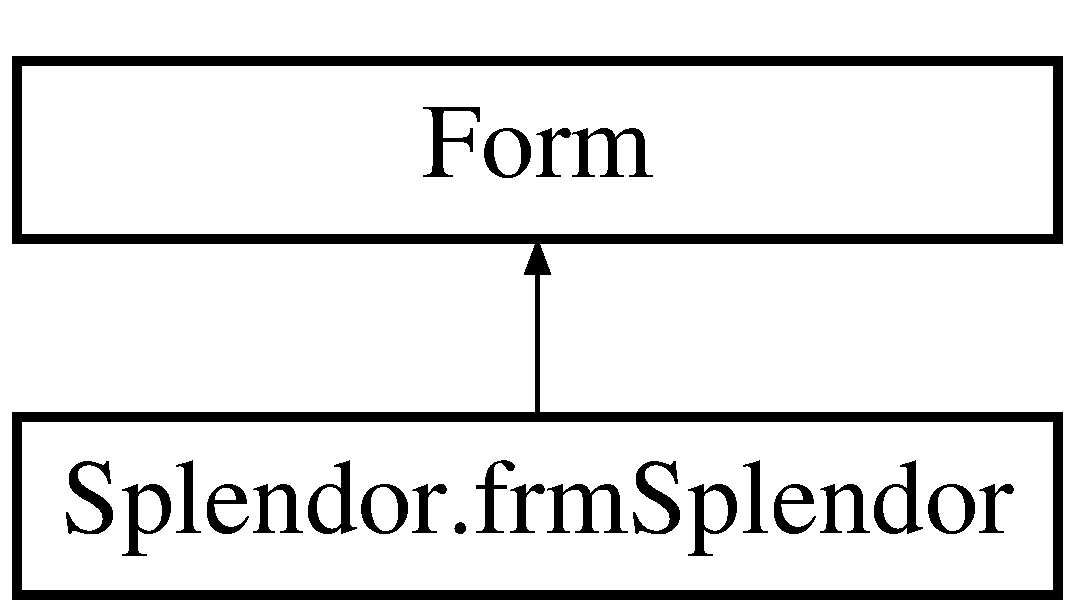
\includegraphics[height=2.000000cm]{class_splendor_1_1frm_splendor}
\end{center}
\end{figure}
\subsection*{Public Member Functions}
\begin{DoxyCompactItemize}
\item 
\mbox{\hyperlink{class_splendor_1_1frm_splendor_ad9c938893d23192acb1996053e3ea87b}{frm\+Splendor}} ()
\begin{DoxyCompactList}\small\item\em constructor \end{DoxyCompactList}\end{DoxyCompactItemize}
\subsection*{Public Attributes}
\begin{DoxyCompactItemize}
\item 
\mbox{\Hypertarget{class_splendor_1_1frm_splendor_a2d8f5bc8e919f7f6c8bfeacc6360f3af}\label{class_splendor_1_1frm_splendor_a2d8f5bc8e919f7f6c8bfeacc6360f3af}} 
int {\bfseries nb\+Player} = 2
\end{DoxyCompactItemize}
\subsection*{Protected Member Functions}
\begin{DoxyCompactItemize}
\item 
override void \mbox{\hyperlink{class_splendor_1_1frm_splendor_a749f4f1d67c78e74aa1a55aa6fdd754b}{Dispose}} (bool disposing)
\begin{DoxyCompactList}\small\item\em Nettoyage des ressources utilisées. \end{DoxyCompactList}\end{DoxyCompactItemize}


\subsection{Detailed Description}
manages the form that enables to play with the \mbox{\hyperlink{namespace_splendor}{Splendor}} 



\subsection{Constructor \& Destructor Documentation}
\mbox{\Hypertarget{class_splendor_1_1frm_splendor_ad9c938893d23192acb1996053e3ea87b}\label{class_splendor_1_1frm_splendor_ad9c938893d23192acb1996053e3ea87b}} 
\index{Splendor\+::frm\+Splendor@{Splendor\+::frm\+Splendor}!frm\+Splendor@{frm\+Splendor}}
\index{frm\+Splendor@{frm\+Splendor}!Splendor\+::frm\+Splendor@{Splendor\+::frm\+Splendor}}
\subsubsection{\texorpdfstring{frm\+Splendor()}{frmSplendor()}}
{\footnotesize\ttfamily Splendor.\+frm\+Splendor.\+frm\+Splendor (\begin{DoxyParamCaption}{ }\end{DoxyParamCaption})}



constructor 



\subsection{Member Function Documentation}
\mbox{\Hypertarget{class_splendor_1_1frm_splendor_a749f4f1d67c78e74aa1a55aa6fdd754b}\label{class_splendor_1_1frm_splendor_a749f4f1d67c78e74aa1a55aa6fdd754b}} 
\index{Splendor\+::frm\+Splendor@{Splendor\+::frm\+Splendor}!Dispose@{Dispose}}
\index{Dispose@{Dispose}!Splendor\+::frm\+Splendor@{Splendor\+::frm\+Splendor}}
\subsubsection{\texorpdfstring{Dispose()}{Dispose()}}
{\footnotesize\ttfamily override void Splendor.\+frm\+Splendor.\+Dispose (\begin{DoxyParamCaption}\item[{bool}]{disposing }\end{DoxyParamCaption})\hspace{0.3cm}{\ttfamily [protected]}}



Nettoyage des ressources utilisées. 


\begin{DoxyParams}{Parameters}
{\em disposing} & true si les ressources managées doivent être supprimées ; sinon, false.\\
\hline
\end{DoxyParams}


The documentation for this class was generated from the following files\+:\begin{DoxyCompactItemize}
\item 
Splendor/Frm\+Splendor.\+cs\item 
Splendor/Frm\+Splendor.\+Designer.\+cs\end{DoxyCompactItemize}

\hypertarget{class_splendor_1_1_player}{}\section{Splendor.\+Player Class Reference}
\label{class_splendor_1_1_player}\index{Splendor.\+Player@{Splendor.\+Player}}


class \mbox{\hyperlink{class_splendor_1_1_player}{Player}} \+: attributes and methods to deal with a player  


\subsection*{Properties}
\begin{DoxyCompactItemize}
\item 
string \mbox{\hyperlink{class_splendor_1_1_player_a15abd489e523e11b6beb4b186783e47f}{Name}}\hspace{0.3cm}{\ttfamily  \mbox{[}get, set\mbox{]}}
\begin{DoxyCompactList}\small\item\em name of the player \end{DoxyCompactList}\item 
int \mbox{[}$\,$\mbox{]} \mbox{\hyperlink{class_splendor_1_1_player_a1c5ccd2470e3bbc84e9a156bc323bfd0}{Ressources}}\hspace{0.3cm}{\ttfamily  \mbox{[}get, set\mbox{]}}
\begin{DoxyCompactList}\small\item\em all the precious stones he has \end{DoxyCompactList}\item 
int \mbox{[}$\,$\mbox{]} \mbox{\hyperlink{class_splendor_1_1_player_a729fa09f28e378e7934f3ae54ea463e9}{Coins}}\hspace{0.3cm}{\ttfamily  \mbox{[}get, set\mbox{]}}
\begin{DoxyCompactList}\small\item\em all the coins he has \end{DoxyCompactList}\item 
int \mbox{\hyperlink{class_splendor_1_1_player_a5616e3562be3e8800f9e959e7cf75194}{Id}}\hspace{0.3cm}{\ttfamily  \mbox{[}get, set\mbox{]}}
\begin{DoxyCompactList}\small\item\em id of the player \end{DoxyCompactList}\item 
\mbox{\Hypertarget{class_splendor_1_1_player_ad92459d327fa7cc546259931af417aa1}\label{class_splendor_1_1_player_ad92459d327fa7cc546259931af417aa1}} 
int {\bfseries Nb\+Prestige}\hspace{0.3cm}{\ttfamily  \mbox{[}get, set\mbox{]}}
\end{DoxyCompactItemize}


\subsection{Detailed Description}
class \mbox{\hyperlink{class_splendor_1_1_player}{Player}} \+: attributes and methods to deal with a player 



\subsection{Property Documentation}
\mbox{\Hypertarget{class_splendor_1_1_player_a729fa09f28e378e7934f3ae54ea463e9}\label{class_splendor_1_1_player_a729fa09f28e378e7934f3ae54ea463e9}} 
\index{Splendor\+::\+Player@{Splendor\+::\+Player}!Coins@{Coins}}
\index{Coins@{Coins}!Splendor\+::\+Player@{Splendor\+::\+Player}}
\subsubsection{\texorpdfstring{Coins}{Coins}}
{\footnotesize\ttfamily int \mbox{[}$\,$\mbox{]} Splendor.\+Player.\+Coins\hspace{0.3cm}{\ttfamily [get]}, {\ttfamily [set]}}



all the coins he has 

\mbox{\Hypertarget{class_splendor_1_1_player_a5616e3562be3e8800f9e959e7cf75194}\label{class_splendor_1_1_player_a5616e3562be3e8800f9e959e7cf75194}} 
\index{Splendor\+::\+Player@{Splendor\+::\+Player}!Id@{Id}}
\index{Id@{Id}!Splendor\+::\+Player@{Splendor\+::\+Player}}
\subsubsection{\texorpdfstring{Id}{Id}}
{\footnotesize\ttfamily int Splendor.\+Player.\+Id\hspace{0.3cm}{\ttfamily [get]}, {\ttfamily [set]}}



id of the player 

\mbox{\Hypertarget{class_splendor_1_1_player_a15abd489e523e11b6beb4b186783e47f}\label{class_splendor_1_1_player_a15abd489e523e11b6beb4b186783e47f}} 
\index{Splendor\+::\+Player@{Splendor\+::\+Player}!Name@{Name}}
\index{Name@{Name}!Splendor\+::\+Player@{Splendor\+::\+Player}}
\subsubsection{\texorpdfstring{Name}{Name}}
{\footnotesize\ttfamily string Splendor.\+Player.\+Name\hspace{0.3cm}{\ttfamily [get]}, {\ttfamily [set]}}



name of the player 

\mbox{\Hypertarget{class_splendor_1_1_player_a1c5ccd2470e3bbc84e9a156bc323bfd0}\label{class_splendor_1_1_player_a1c5ccd2470e3bbc84e9a156bc323bfd0}} 
\index{Splendor\+::\+Player@{Splendor\+::\+Player}!Ressources@{Ressources}}
\index{Ressources@{Ressources}!Splendor\+::\+Player@{Splendor\+::\+Player}}
\subsubsection{\texorpdfstring{Ressources}{Ressources}}
{\footnotesize\ttfamily int \mbox{[}$\,$\mbox{]} Splendor.\+Player.\+Ressources\hspace{0.3cm}{\ttfamily [get]}, {\ttfamily [set]}}



all the precious stones he has 



The documentation for this class was generated from the following file\+:\begin{DoxyCompactItemize}
\item 
Splendor/Player.\+cs\end{DoxyCompactItemize}

%--- End generated contents ---

% Index
\backmatter
\newpage
\phantomsection
\clearemptydoublepage
\addcontentsline{toc}{chapter}{Index}
\printindex

\end{document}
